\section{LLC Converter Design Background}\label{sec:LLC}

As the topology and operating principles of LLC converters are well-established \cite{Wei2021}\cite{Kundu2017}, this section provides a brief overview of the design considerations relevant to the proposed data-driven approach.

For the purposes of this paper, a series resonant converter using a full-bridge inverter and full-bridge synchronous rectifier with an LLC tank was chosen due to its ability to achieve both zero current and zero voltage switching.
The chosen circuit schematic can be seen in Figure~\ref{fig:llcsrc}.

\begin{figure}[h]
	\centering
	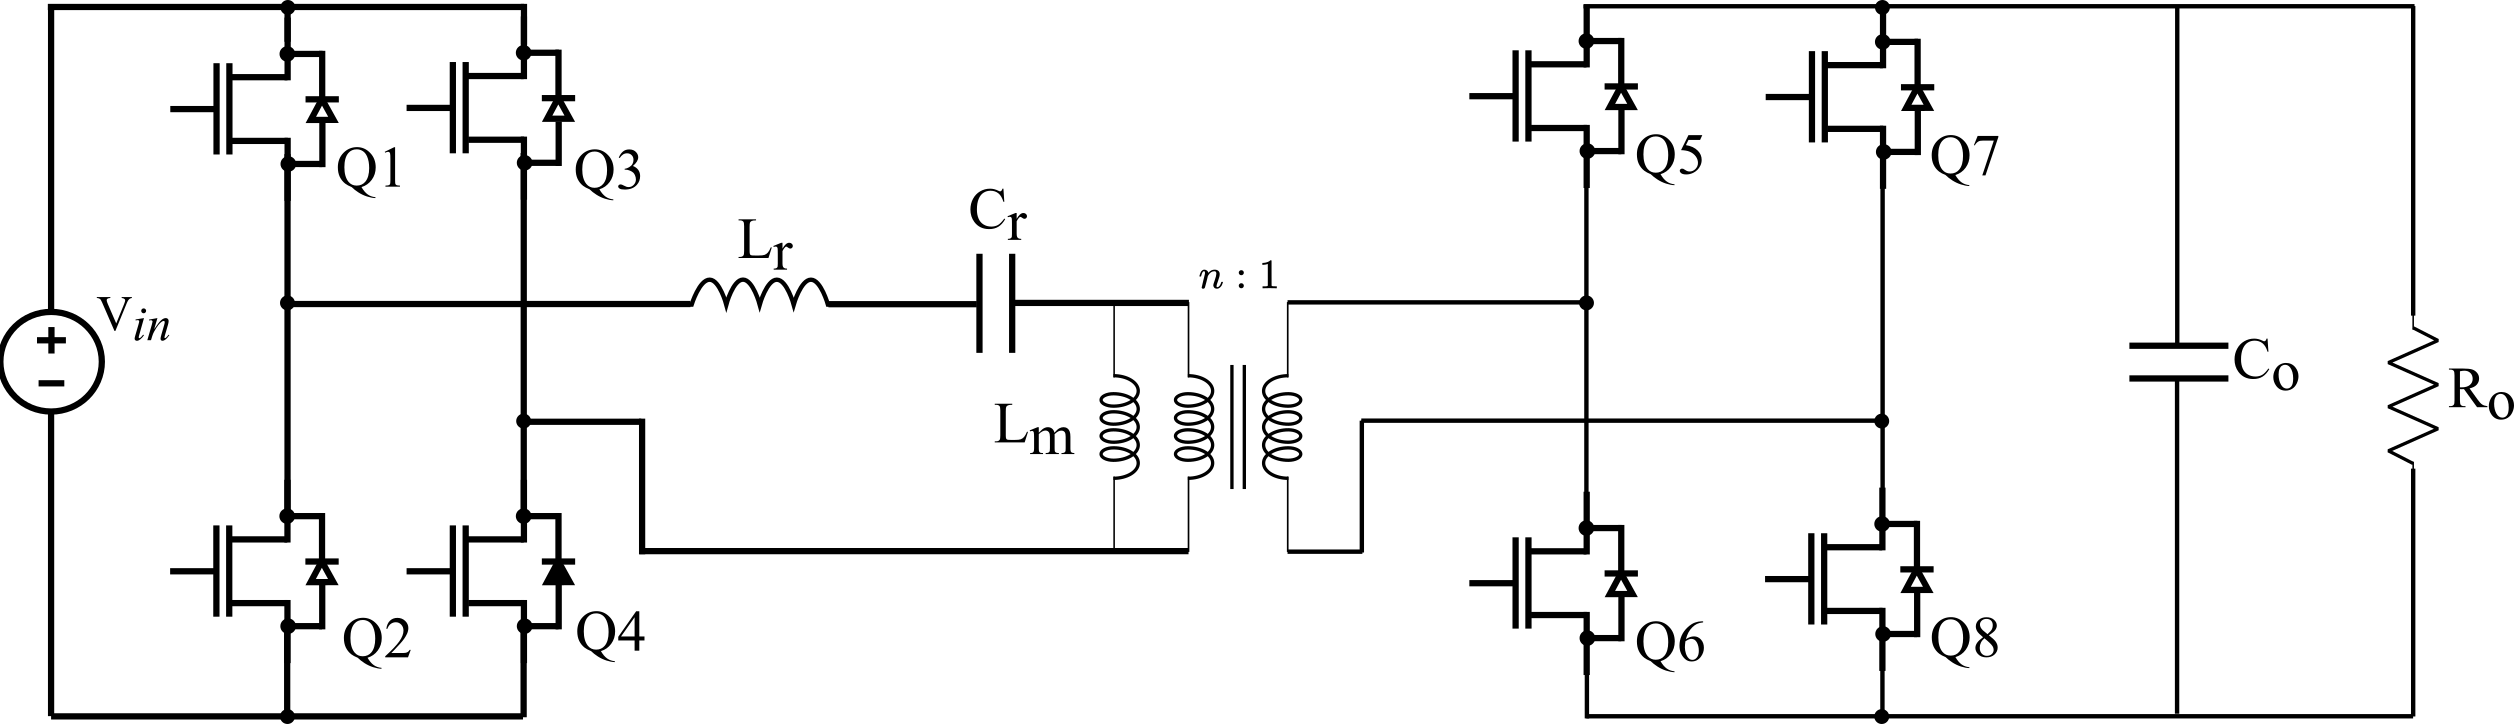
\includegraphics[width=\columnwidth]{figures/LLCSR.png}
	\caption{The initial circuit schematic for the series resonant LLC converter.}
	\label{fig:llcsrc}
\end{figure}

To generate initial training data for the machine learning model, a converter using this topology was designed using the traditional first harmonic approximation (FHA) method \cite{Jung2007}.
Under these assumptions, the circuit simplifies to the layout in Fig.~\ref{fig:llcfha-3}.

\begin{figure}[h]
	\centering
	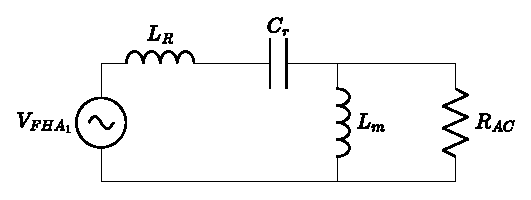
\includegraphics[width=.75\columnwidth]{figures/LLC_FHA-3}
	\caption{The simplified converter topology under the first harmonic approximation}
	\label{fig:llcfha-3}
\end{figure}

Under the assumption that the first harmonic contributed by the source is dominant, the gain of the converter can be derived as a voltage division between the load resistance in parallel with the transformer magnetizing inductance and the series tank impedance.
\begin{align}
	M &= \frac{V_{out}}{V_{in}}= \left|\frac{Z_{L_m}//R_{AC}} {Z_{L_m} // R_{AC} + Z_{L_r} + Z_{C_r}} \right|
\end{align}

\begin{align}
	M &= \left| \frac{\left((j\omega L_m)^{-1} + R_{AC}^{-1}\right)^{-1}}{\left((j\omega L_m)^{-1} + R_{AC}^{-1}\right)^{-1} + j\omega L_r - \frac{j}{\omega C_r}} \right|\\
	&= \frac{f^{\prime^2}k}{\sqrt{\left[(k+1)f^{\prime^2}-1\right]^2+\left[Qkf^\prime(f^{\prime^2}-1)\right]^2}}
\end{align}


where $M$ is the converter Gain, $Z_{L_m}$ is the magnetizing inductance, $Z_{L_r}$ is the resonant inductance, $Z_{C_r}$ is the resonant capacitance, $f^\prime$ is the normalized frequency, $k$ is the inductance ratio, and $R_{AC}$ is the reflected load resistance, $V_{in}$ is the input voltage, $V_{out}$ is the output voltage, and $Q$ is the quality factor.

\[Q = \frac{\sqrt{L_r/C_r}}{R_{AC}}\quad f^\prime = \frac{f_{sw}}{f_r}\quad k = \frac{L_m}{L_r}\quad R_{AC}=\frac{8n^2}{\pi^2}R\]

where $n$ is the transformer turns ratio, $f_{sw}$ is the switching frequency, $f_r$ is the resonant frequency, and $R$ is the load resistance.

From here, knowing the desired gain, a transformer winding ratio can be chosen to ease the gain required by the resonant tank.
With a known turns ratio, choose an applicable quality factor "Q" based on anticipated loading and determine the final gain by picking the resonant inductor value.

\begin{figure}[h]
	\centering
	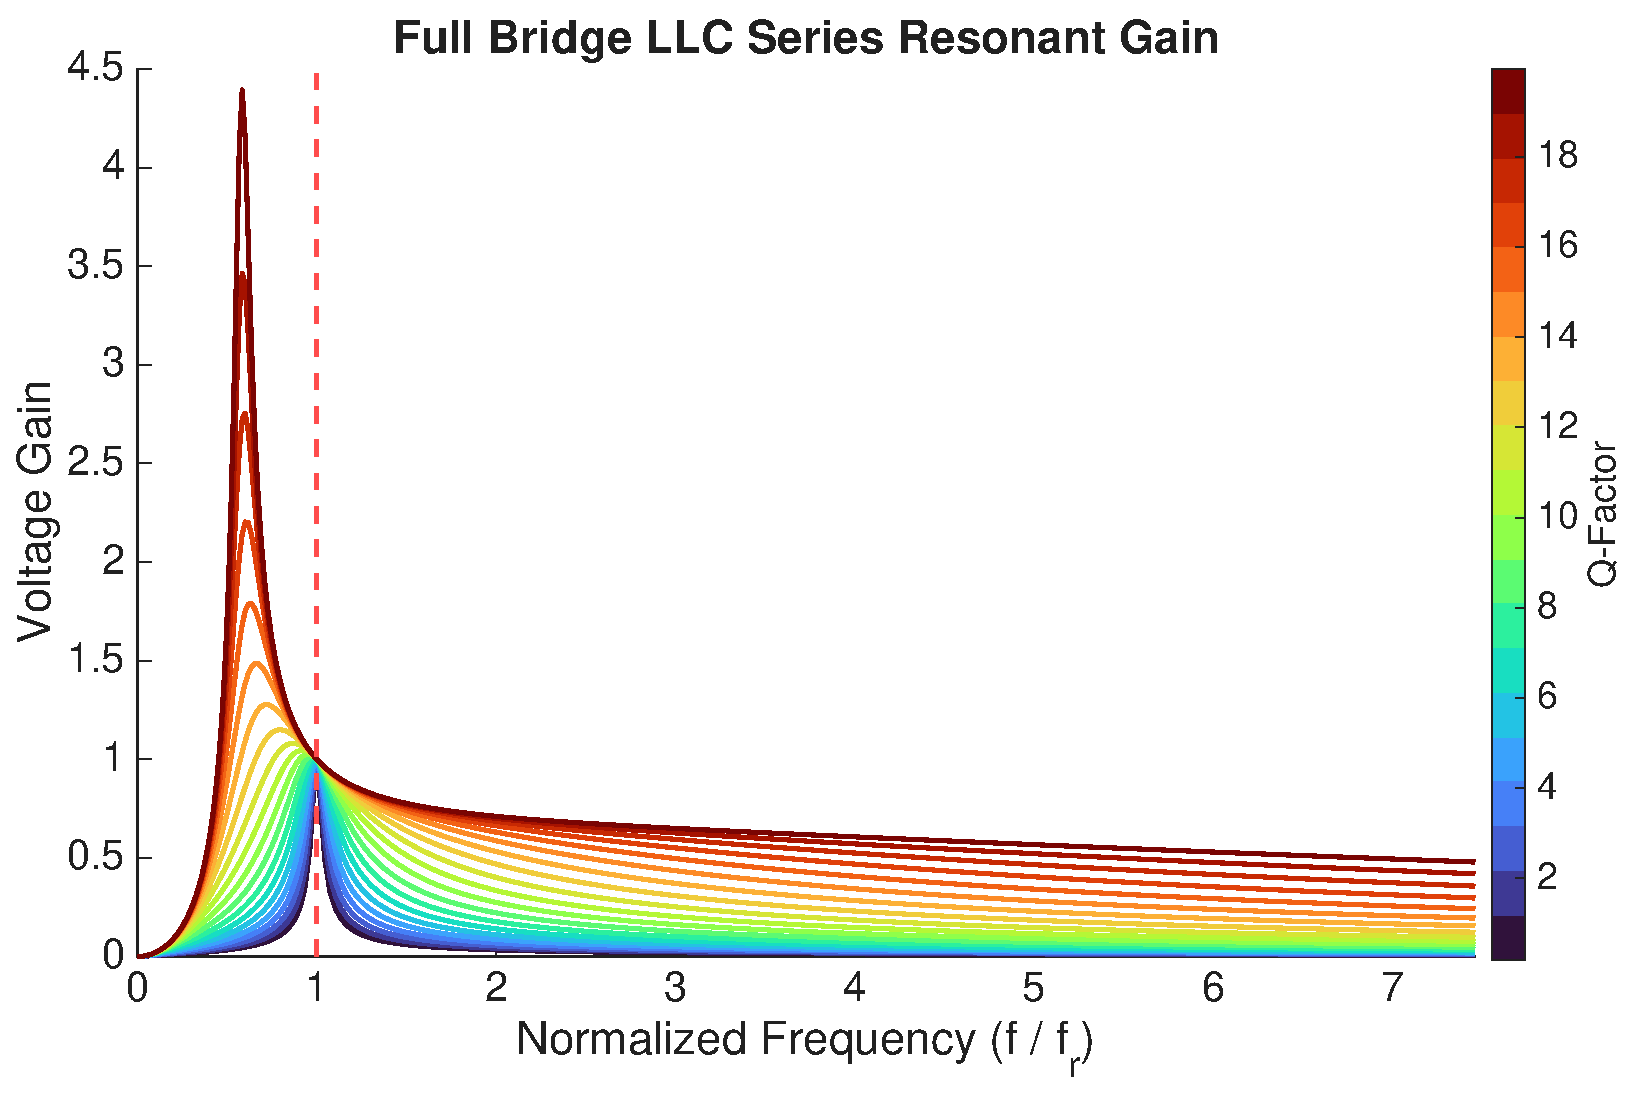
\includegraphics[width=\columnwidth]{figures/gain_q_sweep}
	\caption{Converter gain as a function of switching frequency and quality factor}
	\label{fig:gain_q_sweep}
\end{figure}

Finally, ensure that the desired performance is achievable using the selected component ratings, including the transformer and magnetizing inductance design. Although the conventional FHA-based design procedure provides useful analytical insight, the overall process remains inherently iterative, often requiring repeated converter simulations and parameter adjustments between component selections. In addition, the accuracy of the FHA approach is generally highest near the resonant operating frequency, where LLC converters are typically designed to operate. These limitations motivate the development of the proposed data-driven framework, which enables rapid evaluation of the design space while reducing the dependence on repeated time-domain simulations during the optimization stage.